\section{引言}



近期，大型语言模型（LLM）在显式思维链（CoT）推理任务上展现出色表现~\citep{wei2022chain,wang2022self,kojima2022large,qin2024large}，但它们依旧难以从指令微调模型或基座模型“冷启动”出需要长序列、多阶段推理的长链式思维链（Long CoT）能力~\citep{chen2025towards,chen-etal-2025-unveiling-key}。值得注意的是，\citet{du2025the} 指出，人类能够在不模仿 DeepSeek-R1~\citep{guo2025deepseek} 的情况下生成 Long CoT 理由。我们在预研阶段发现，使用人类或指令模型的推理轨迹（在随机采样的 Long CoT 样本上）进行标准监督微调或蒸馏，并不能可靠地把这些能力注入 LLM：模型不是在长轨迹中失去连贯性，就是无法把模式迁移到新任务上。这引出了一个核心问题：

\begin{quotation}
{\begin{center}
    \textbf{大型语言模型究竟如何学习并表征有效的长链式思维链？}
\end{center}}
\end{quotation}



\begin{figure*}[t]
    \centering
    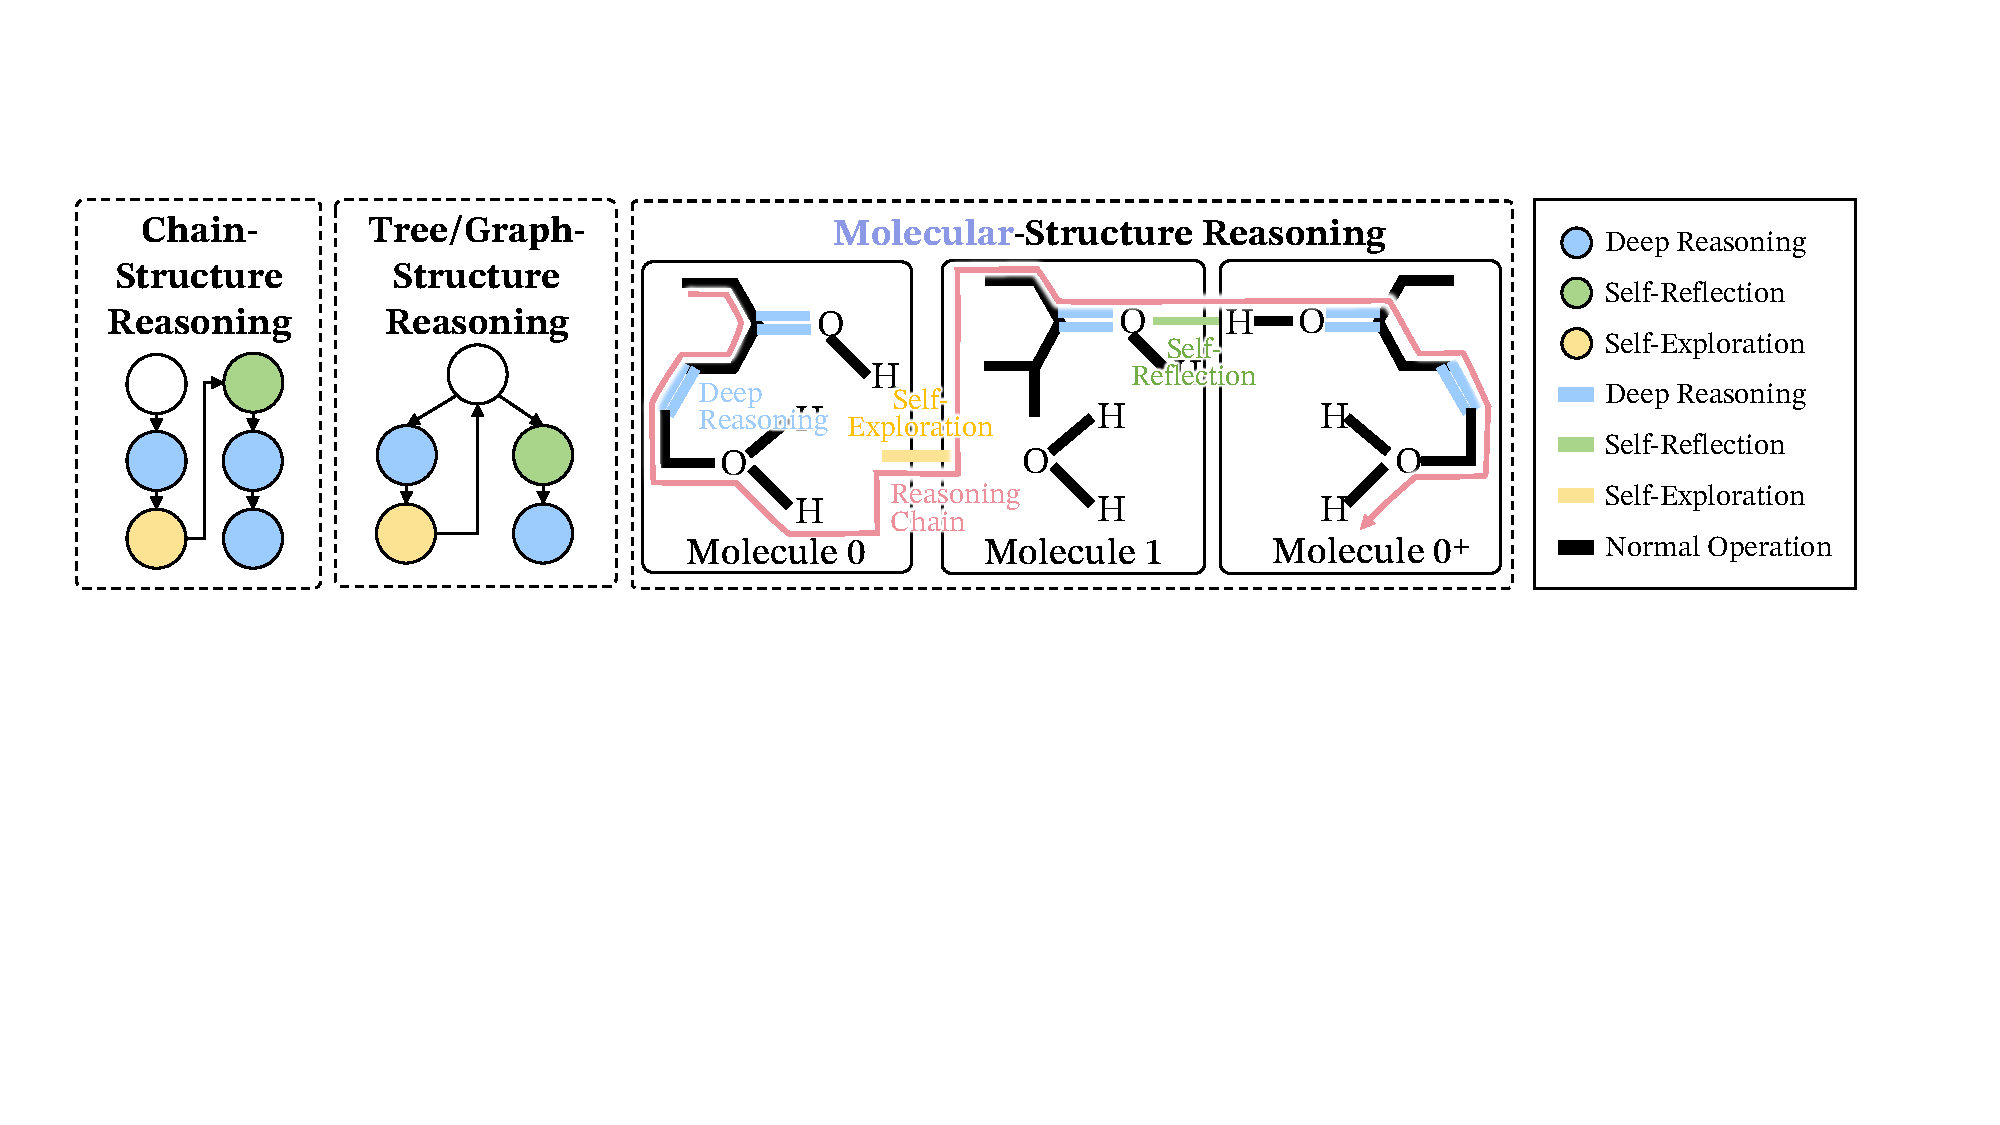
\includegraphics[width=0.98\textwidth]{figures/intro.pdf}
    \caption{以往工作多把推理建模为链状或树状节点，我们则提出“分子结构”视角。推理在 Mole. 0 起步，先在强相关结构上进行\textbf{深层推理}，再借助\textbf{自我探索}扩展到新逻辑（Mole. 1）；当遇到错误时，再以\textbf{自我反思}将链条折返并优化为 Mole. 0$^{+}$。}
    
    \label{fig:intro}
\end{figure*}


为解释这一现象，我们认为模型其实在习得“推理轨迹的组织结构”。如图~\ref{fig:intro} 所示，既有研究通常把轨迹建模为由逻辑节点组成的序列或树。然而，我们对多个强推理模型的 Long CoT 分析显示：跨任务、跨架构地存在三类核心行为的稳定分布——深层推理、自我反思、自我探索~\citep{chen2025towards}；而单纯的节点视角无法捕捉这一分布特征。

这一发现启发我们采用类似分子、聚合物的分布视角：把带有行为标签的\emph{逻辑边}看作交互键，并研究其全局的\textbf{分子结构}如何确保长程推理的稳定性。具体而言，深层推理像共价键一样形成密集的局部耦合推理片段；自我反思类似氢键，负责把后续步骤与早期步骤远程纠偏地连接起来；自我探索则像范德华力，为不同推理团簇之间提供松散的桥接。因此，高质量的 Long CoT 本质上来源于这些“键类型”的\textbf{稳定组成和排列}，它们决定了模型是否能高效学习\footnote{本文提及的元素符号 C、H、O 仅为类比说明分子结构，不具备化学含义。}。

在该框架下，我们把“语义异构体”定义为：在同一任务上访问相似语义区域、但行为分布与转移准则不同的 Long CoT 轨迹。我们证明，对于同一类任务往往存在多个近似最优的语义异构体；然而，当把来自不同强师模型的稳定异构体混合在一起时，学习过程会被破坏，即便它们在 token 统计上匹配，性能和行为分布仍然会显著退化。这也从结构层面解释了为什么简单拼接异构 Long CoT 轨迹经常失败，而不仅仅是 token 层面的蒸馏问题。

基于上述视角，我们提出了 \method：一种关注结构的合成框架。它首先从强推理模型估计行为转移图，然后引导指令模型以受控方式合成新的推理轨迹，以迁移这种“行为结构”，而不是直接拷贝教师输出。这样，我们可以把结构迁移与具体表面形式解耦：模型能够从零开始生成匹配目标行为分布的 Long CoT 数据，并在多个基准上带来稳定的推理收益和强化学习稳定性提升。

随后，我们分析每种“键”在 Long CoT 结构中的塑形作用：深层推理键负责编码核心逻辑流程；自我反思键帮助轨迹折返并回溯前序步骤；自我探索键则维持远程一致性检查，使得我们可以面向具体任务分配所需的键分布。此外，我们还讨论为什么一旦分子结构被破坏就难以恢复：这解释了私有 LLM 如何通过蒸馏防护来保护内生的长链结构。诸如摘要、思路压缩等方法会打乱 Long CoT 结构，因此阻止了对真实推理过程的未授权复制。

总结来说，本文的贡献包括：
\begin{itemize}[leftmargin=16pt, itemsep=0pt, topsep=0pt]
\item 我们把 Long CoT 建模为由三类键组成的分子结构：深层推理（共价键）、自我反思（氢键）与自我探索（范德华力），据此刻画其有效学习机制；
\item 我们提出“有效语义异构体”，说明仅有促使熵快速收敛的键型才能带来稳定学习，而结构互相竞争会破坏训练；
\item 我们提出 \method，通过分布迁移图来合成这些结构，从而在 6 个基准上全面提升 Long CoT 表现并稳定强化学习。
\end{itemize}
